\documentclass[11pt]{report}
\usepackage{tikz}
\usetikzlibrary{fit,positioning}
\usepackage[labelfont=bf]{caption}

\begin{document}
	
\section*{Exercise 1}	

DAG-representation ...  

\begin{figure}[!htb]
\centering
	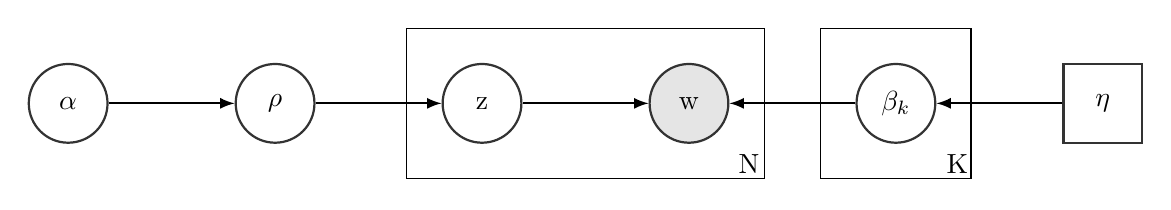
\begin{tikzpicture}
\tikzstyle{main}=[circle, minimum size = 10mm, thick, draw =black!80, node distance = 16mm]
\tikzstyle{rect}=[rectangle, minimum size = 10mm, thick, draw =black!80, node distance = 16mm]
\tikzstyle{connect}=[-latex, thick]
\tikzstyle{box}=[rectangle, draw=black!100]
  \node[main, fill = white!100] (alpha) [label=center:$\alpha$] { };
  \node[main] (rho) [right=of alpha,label=center:$\rho$] { };
  \node[main] (z) [right=of rho,label=center:z] {};
  \node[main, fill = black!10] (w) [right=of z,label=center:w] { };
  \node[main] (beta) [right=of w,label=center:$\beta_k$] { };
  \node[rect] (eta) [right=of beta,label=center:$\eta$] { };
  \path (alpha) edge [connect] (rho)
        (rho) edge [connect] (z)
        (z) edge [connect] (w)
        (eta) edge [connect] (beta)
        (beta) edge [connect] (w);
  \node[rectangle, inner sep=0mm, fit= (z) (w),label=below right:N, xshift=13mm] {};
  \node[rectangle, inner sep=4.4mm,draw=black!100, fit= (z) (w)] {};
 % \node[rectangle, inner sep=4.6mm, fit= (z) (w),label=below right:M, xshift=12.5mm] {};
  %\node[rectangle, inner sep=9mm, draw=black!100, fit =  (z) (w)] {};
   \node[rectangle, inner sep=4.4mm,draw=black!100, fit= (beta)] {};
  \node[rectangle, inner sep=0mm,fit= (beta),label=below right:K, xshift=0mm] {};
\end{tikzpicture}
\caption{DAG Representation}
\end{figure}


\end{document}
%note - compiled with pdflatex